% Figure 2: two stacked ablation panels (data = what the course scripts print)
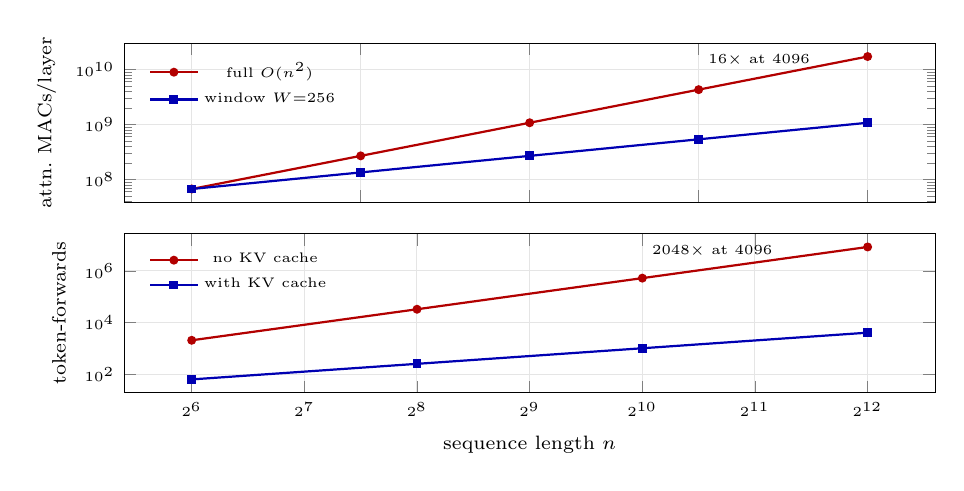
\begin{tikzpicture}
\begin{axis}[
  name=attn,
  width=0.98\columnwidth, height=3.6cm,
  xmode=log, ymode=log, log basis x=2,
  xlabel={}, ylabel={attn.\ MACs/layer},
  xticklabels={},
  legend style={font=\tiny, at={(0.02,0.95)}, anchor=north west, draw=none, fill=none},
  tick label style={font=\tiny}, label style={font=\scriptsize},
  grid=major, grid style={gray!20},
]
\addplot[color=red!70!black, mark=*, mark size=1.2pt, thick]
  coordinates {(256,67108864)(512,268435456)(1024,1073741824)(2048,4294967296)(4096,17179869184)};
\addlegendentry{full $O(n^2)$}
\addplot[color=blue!70!black, mark=square*, mark size=1.2pt, thick]
  coordinates {(256,67108864)(512,134217728)(1024,268435456)(2048,536870912)(4096,1073741824)};
\addlegendentry{window $W{=}256$}
\node[font=\tiny, anchor=west] at (axis cs:2048,15000000000) {$16\times$ at 4096};
\end{axis}
\begin{axis}[
  at={(attn.south west)}, anchor=north west, yshift=-4mm,
  width=0.98\columnwidth, height=3.6cm,
  xmode=log, ymode=log, log basis x=2,
  xlabel={sequence length $n$}, ylabel={token-forwards},
  legend style={font=\tiny, at={(0.02,0.95)}, anchor=north west, draw=none, fill=none},
  tick label style={font=\tiny}, label style={font=\scriptsize},
  grid=major, grid style={gray!20},
]
\addplot[color=red!70!black, mark=*, mark size=1.2pt, thick]
  coordinates {(64,2080)(256,32896)(1024,524800)(4096,8390656)};
\addlegendentry{no KV cache}
\addplot[color=blue!70!black, mark=square*, mark size=1.2pt, thick]
  coordinates {(64,64)(256,256)(1024,1024)(4096,4096)};
\addlegendentry{with KV cache}
\node[font=\tiny, anchor=west] at (axis cs:1024,6000000) {$2048\times$ at 4096};
\end{axis}
\end{tikzpicture}
